
\documentclass[10pt]{article}
\usepackage{multicol}
\usepackage{geometry}
\geometry{bottom=4em,top=6em, inner=2.2cm, outer=4em,  headheight=\paperheight}
\usepackage[export]{adjustbox}
\usepackage{array}
\usepackage{amsmath}
\usepackage{amsfonts}
\usepackage{fancyhdr}
\usepackage{lastpage}
\usepackage{xcolor}
\usepackage{enumitem}
\usepackage{pifont}
\usepackage{graphicx}
\graphicspath{{../img}}
\usepackage{pgfplots}
\pgfplotsset{compat=1.18}
\usepackage{tabularx}
\usepackage{polynom}
\usepackage{setspace}
\usepackage{pdfpages}
\usepackage{tikz}
\usetikzlibrary{angles,quotes}
\setlist{nosep}

\pagestyle{empty}

\begin{document}

\begin{center}
{\Large\textbf{TI-84 Regression Cheat Sheet}}
\end{center}

\begin{multicols}{2}

\section*{1. Enter the Data}

\begin{enumerate}
\item Press \texttt{STAT}
\item Select \texttt{1:Edit}
\item Enter $x$ values in \texttt{L1}
\item Enter $y$ values in \texttt{L2}
\end{enumerate}

\section*{2. Turn On Correlation Coefficient}

(Do this once.)

\begin{enumerate}
\item \texttt{2nd} \texttt{0}
\item Select \texttt{DiagnosticOn}
\item Press \texttt{ENTER} twice
\end{enumerate}

\section*{3. Linear Regression}

Use when data changes by about the same amount each step.

\begin{enumerate}
\item \texttt{STAT}
\item \texttt{CALC}
\item \texttt{4:LinReg(ax+b)}
\item Enter \texttt{L1,L2}
\item \texttt{ENTER}
\end{enumerate}

Calculator gives:

\[
y=ax+b
\]

Write the equation exactly.

Example:

\[
a=2.5,\quad b=7
\]

\[
\boxed{y=2.5x+7}
\]

\section*{4. Exponential Regression}

Use when data grows or decays by about the same percent.

\begin{enumerate}
\item \texttt{STAT}
\item \texttt{CALC}
\item \texttt{0:ExpReg}
\item Enter \texttt{L1,L2}
\item \texttt{ENTER}
\end{enumerate}

Calculator gives:

\[
y=ab^x
\]

Example:

\[
a=120,\quad b=1.08
\]

\[
\boxed{y=120(1.08)^x}
\]

\columnbreak

\section*{5. Make Predictions}

Substitute the given $x$ value into the regression equation.

Example:

\[
y=2.5x+7
\]

When $x=10$:

\[
y=2.5(10)+7=32
\]

\section*{6. Correlation Coefficient}

The calculator displays $r$ after \texttt{LinReg}.

\vspace{0.3em}

\begin{tabular}{|c|c|}
\hline
$r$ & Meaning\\
\hline
Near $1$ & Strong Positive\\
\hline
Near $-1$ & Strong Negative\\
\hline
Near $0$ & Weak/None\\
\hline
\end{tabular}

\vspace{0.5em}

Regents shortcut:

\[
|r| \approx 1
\]

Good fit

\[
|r| \approx 0
\]

Poor fit

\section*{7. Regents Strategy}

\begin{enumerate}
\item Put data in L1 and L2.
\item Run the requested regression.
\item Copy the equation.
\item Use the equation to predict values.
\item Use $r$ if asked about correlation.
\end{enumerate}

\section*{Memorize}

\[
\boxed{\text{Linear: } y=ax+b}
\]

\[
\boxed{\text{Exponential: } y=ab^x}
\]

\[
\boxed{|r|\text{ close to }1
\Rightarrow
\text{strong correlation}}
\]

\end{multicols}
\clearpage
{\bf Linear Regression}

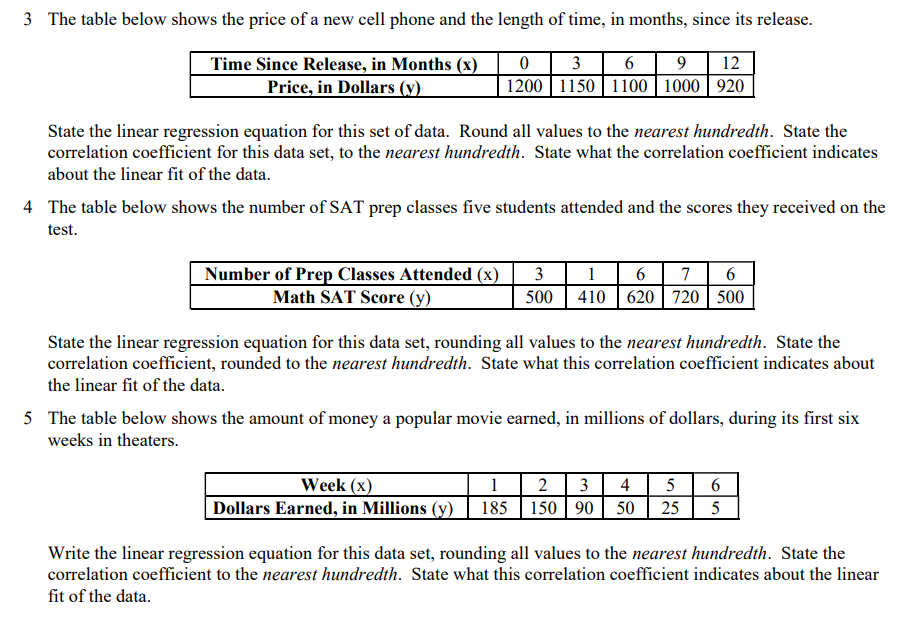
\includegraphics[width=.8\textwidth, height=0.4\paperheight]{regents_linear_regression.png}

{\bf Exponential Regression}

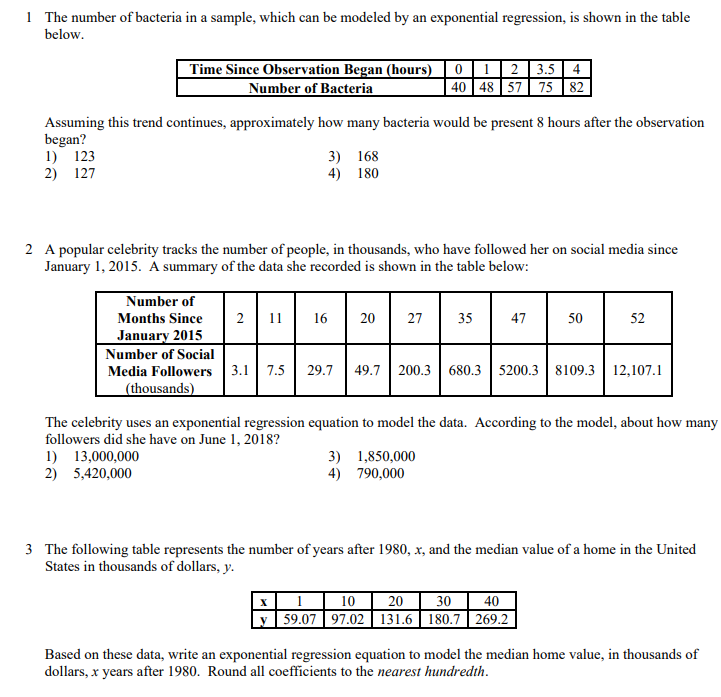
\includegraphics[width=.8\textwidth,height=0.4\paperheight]{regents_exponential_regression.png}
\end{document}

